%% LyX 2.1.4 created this file.  For more info, see http://www.lyx.org/.
%% Do not edit unless you really know what you are doing.
\documentclass[12pt,english]{report}
\usepackage[T1]{fontenc}
\usepackage[latin9]{inputenc}
\usepackage{babel}
\usepackage{longtable}
\usepackage{float}
\usepackage{calc}
\usepackage{amsmath}
\usepackage{amsthm}
\usepackage{setspace}
\usepackage[unicode=true,pdfusetitle,
 bookmarks=true,bookmarksnumbered=false,bookmarksopen=false,
 breaklinks=false,pdfborder={0 0 1},backref=false,colorlinks=false]
 {hyperref}

\makeatletter

%%%%%%%%%%%%%%%%%%%%%%%%%%%%%% LyX specific LaTeX commands.
\providecommand{\LyX}{\texorpdfstring%
  {L\kern-.1667em\lower.25em\hbox{Y}\kern-.125emX\@}
  {LyX}}
%% Because html converters don't know tabularnewline
\providecommand{\tabularnewline}{\\}
\floatstyle{ruled}
\newfloat{algorithm}{tbp}{loa}[chapter]
\providecommand{\algorithmname}{Algorithm}
\floatname{algorithm}{\protect\algorithmname}

%%%%%%%%%%%%%%%%%%%%%%%%%%%%%% Textclass specific LaTeX commands.
\usepackage{UTSAthesis}      
\usepackage{times}            
\usepackage{latexsym}

%Bibliography packages
\usepackage[square]{natbib} % defines citet, citep, ...
\bibpunct{(}{)}{;}{a}{}{,} % to follow the A&A style - 
\newcommand{\aj}{AJ}
\newcommand{\apj}{ApJ}
\newcommand{\apjl}{ApJ}
\newcommand{\apjs}{ApJS}
\newcommand{\aap}{A\&A}
\newcommand{\aaps}{A\&AS}
\newcommand{\mnras}{MNRAS}
\newcommand{\nat}{Nature}
\newcommand{\araa}{ARAA}
\newcommand{\prd}{Phys. Rev. D}
\newcommand{\pasj}{PASJ}
\newcommand{\ETC}{et al.}
\newcommand{\physrep}{Physics Report}
\newcommand{\gca}{GCA}
\newcommand{\pasa}{PASA}
\newcommand{\pasp}{PASP}
\newcommand{\aapr}{A\&A~Rev.}
\newcommand{\apss}{Ap\&SS}
%End of bibliography packages 

%Added by me
\newcommand\numberthis{\addtocounter{equation}{1}\tag{\theequation}}
%End of added by me

\newenvironment{ruledcenter}{%
  \begin{center}
  \rule{\textwidth}{1mm} } {%
  \rule{\textwidth}{1mm} 
  \end{center}}%


  \theoremstyle{definition}
  \newtheorem{defn}{\protect\definitionname}
\theoremstyle{plain}
\newtheorem{thm}{\protect\theoremname}

\@ifundefined{showcaptionsetup}{}{%
 \PassOptionsToPackage{caption=false}{subfig}}
\usepackage{subfig}
\makeatother

  \providecommand{\definitionname}{Definition}
\providecommand{\theoremname}{Theorem}

\begin{document}

% Committee Members
\supervisor{Mario Diaz, Ph.D.}
\committeeB{Lucas Macri, Ph.D.}
\committeeC{Matthew Benacquista, Ph.D.}
\committeeD{Eric Schlegel, Ph.D.}
\committeeE{Ricardo Lopez Mobilia, Ph.D.}

\informationitems{Doctor of Philosophy in Physics}{Ph.D.}{M.Sc.}{Department of Physics And Astronomy}{College of Sciences}{May}{ 2017 }

\thesiscopyright{Copyright 2017 Martin Beroiz \\
All rights reserved. }

\dedication{\emph{I would like to dedicate this thesis to ??????.}}


\title{OPTICAL COUNTERPARTS TO GRAVITATIONAL WAVES}


\author{Martin Beroiz}
\maketitle
\begin{acknowledgements}
Thanks y'all.

(Notice: If any part of the thesis/dissertation has been published
before, the following two paragraphs should be included without alteration).

\begin{singlespace}
\emph{This Masters Thesis/Recital Document or Doctoral Dissertation
was produced in accordance with guidelines which permit the inclusion
as part of the Masters Thesis/Recital Document or Doctoral Dissertation
the text of an original paper, or papers, submitted for publication.
The Masters Thesis/Recital Document or Doctoral Dissertation must
still conform to all other requirements explained in the Guide for
the Preparation of a Masters Thesis/Recital Document or Doctoral Dissertation
at The University of Texas at San Antonio. It must include a comprehensive
abstract, a full introduction and literature review, and a final overall
conclusion. Additional material (procedural and design data as well
as descriptions of equipment) must be provided in sufficient detail
to allow a clear and precise judgment to be made of the importance
and originality of the research reported. }

\emph{It is acceptable for this Masters Thesis/Recital Document or
Doctoral Dissertation to include as chapters authentic copies of papers
already published, provided these meet type size, margin, and legibility
requirements. In such cases, connecting texts, which provide logical
bridges between different manuscripts, are mandatory. Where the student
is not the sole author of a manuscript, the student is required to
make an explicit statement in the introductory material to that manuscript
describing the students contribution to the work and acknowledging
the contribution of the other author(s). The signatures of the Supervising
Committee which precede all other material in the Masters Thesis/Recital
Document or Doctoral Dissertation attest to the accuracy of this statement.}\end{singlespace}
\end{acknowledgements}
\begin{abstract}
The first chapter of this document is a description of the content
and the usage of the UTSAthesis package. The remaining chapters serve
to illustrate some use of \LyX{} features for writing a thesis/dissertation. 

The first line of the abstract has been indented as per required by
the thesis/dissertation guideline.
\end{abstract}

\pageone{}

\chapter{Introduction}

After 100 years after the prediction of gravitational waves (GW from hereon)

\section*{The LIGO Project}
* Lengthy LIGO Description

\section*{Multi-Messenger Astronomy}
* The raise of and need for multi messenger astronomy

\section*{The TOROS Collaboration (or project?)}
* Lengthy TOROS Description (whatever it evolved into at this point)

TOROS, the Transient Optical Robotic Observatory of the South, is a collaboration formed to respond to GW events as detected by the LVC.
Its main purpose then is to detect transient events compatible with expected (or not) signatures of events that can give mutual birth to GW and optical triggers.

Being in its early stages of development, and given the new nature of the multimessenger astronomy, the TOROS team is building up the tools and infrastructure that will make it capable in the future to promptly respond to this alerts.

Several things can enter in consideration for this task, from software development to forging ties with existing observatories. 

My thesis will focus on several challenges in the development of the software infrastructure needed to process the observatory data. 

At the moment of this writing, TOROS Collaboration consists of several astronomical institutions that showed interest in doing a search and possible follow-ups of candidates to interesting events.

The list of participant institutions is as follows: (should I list them?)

At UT Rio Grande Valley, we developed extensive analysis and web code to allow for the interaction between the institutions (just the broker page, really). 



\section*{The Transient World}

\section{The Time-Domain Revolution in Astronomy}
* GW20150914 and our contribution

* The transient world
	* The Time Domain revolution in Astronomy
	* What are transients and which ones are we interested in

	* How can we catch transients
		* Previous work: Catalog Matching: Marica's pipeline and Shuang's work on the transient identification and comparison to my OIS code.
		* Previous work: OIS + ML (the iPTF experience)
		* Subsection on ML (Supervised vs. Unsupervised, overall view and some popular algorithms)
		* Discussion of both methods


\chapter{Difference Image Analysis}

Searches for time-varying and position-changing objects are undertaken by comparing a reference image of a particular region of the sky with a second image taken at the moment in which we are interested. Ideally, the reference image is taken with the same telescope using the same filter and CCD. The two images have to be aligned pixel by pixel and then subtracted to reveal any changes in light.

To make a suitable subtraction of two images, one has to match the frames to exactly the same seeing. Image Difference is a technique to find a convolution kernel that best describes (in some minimization sense) the change in point spread function between the images. The idea is to degrade the good seeing image---our reference image---to match the seeing of our second image. Finding the proper kernel can be a delicate operation and there's plenty of literature on the subject. Methods range from PSF modeling through common Gaussian profiles to unmodeled PSF's to Information Theory and Fourier Domain.

The first attempts at image subtraction relied on Fourier decomposition of the images, 
but the technique suffered when noise levels were even moderate and the results were not always good.
\citet{1998ApJ...503..325A} were the first to propose a solution in image space (as opposed to Fourier space). 
They also summarize previous efforts in their introduction and references therein. 
In that paper, they propose an optimization problem that we describe briefly as follows.

We have an image $I$ and a reference image $R$, for which we want to find a convolution kernel $K$ such that

\begin{align}
I(x,y) & \approx (R \mathbin{*} K)(x,y) \\
 & \approx \int \mathrm{d}u \mathrm{d}v {R (u,v) K(x-u,y-v)}
\end{align}
 
The integral symbol has to be understood in practice, as a sum over all the pixels $(x,y)$ on the image. 

The kernel $K$ will try to correct for the PSF difference between the two images.
It's worth noting here, that even though it could be practical to the reader to think so, the kernel $K$ is neither the PSF of the reference nor the PSF of the image.

Usually, the reference image is the one with the best {\em seeing}, 
because it can be done by median-stacking good images, or using Lucky Imaging [add ref] or some other method.

To convert the problem into a linear one, we decompose the kernel into a linear combination of ``{\em basis}'' functions $B$.

\begin{equation} \label{kernel_linear}
K(u,v) = \sum_{i} a_{i} B_{i}(u,v)
\end{equation}

These $B_{i}$ could in principle be any reasonable set of functions. 
%The two most popular choices are modulated Gaussians and the Delta basis, which will be explained in further detail in section \ref{basis}.

Using this linear combination, the convolution will be

\begin{align}
(R \mathbin{*} K)(x,y) & = \sum_{i} a_{i} \left( R \mathbin{*} B_{i} \right)(x,y) \\
 & \equiv \sum_{i} a_{i} C_{i}(x,y)
\end{align}

where the last line defines $C_{i}(x,y)$.

With this decomposition, we can find the set of $a_{i}$ that minimizes the square difference over all pixels.
Define a cost function $Q$:

\begin{align}
Q &= \int \left( I(x,y) - (R \mathbin{*} K)(x,y) \right)^2 \\
 & = \int \left( I(x,y) - \sum_{i} a_{i} C_{i}(x,y) \right)^2,
\end{align}

and let's minimize $Q$ over the set of $a$'s:

\begin{align}
\frac{\partial Q}{\partial a_{i}} = & 2 \int \left( I(x,y) - \sum_{j} a_{j} C_{j}(x,y) \right) C_{i}(x,y) 
\end{align}

Setting the last equation to zero, gives us:

\begin{align}
\sum_{j} a_{j} \int \left( C_{j}(x,y)  C_{i}(x,y) \right) =  \int I(x,y) C_{i}(x,y) 
\end{align}

Which we can write more succinctly as a matrix equation:

\begin{align} \label{matrix_eq}
\sum_{j} M_{ij} a_{j}  =  b_{i}
\end{align}

where

\begin{align} \label{matrix_def}
M_{ij}  &=   \int  C_{i}(x,y)  C_{j}(x,y) \\
b_{i} &=  \int I(x,y) C_{i}(x,y)  \nonumber
\end{align}

We can find the coefficients $a_{i}$ of the optimal kernel for the subtraction by inverting the system \eqref{matrix_eq}.

\section{Different basis functions}

As stated above, any choice of basis in the linearization \eqref{kernel_linear} could work, but two particular choices are the most popular.

The first one was proposed by \citet{1998ApJ...503..325A} and it consist of modulated centered Gaussians:

\begin{equation}
B_{n,d_n^{x}, d_n^{y}}(u,v) = e^{-(u^2+v^2)/2 \sigma_n^2} \times u^{d_n^{x}} v^{d_n^{y}}
\end{equation}

where the exponents in $u$ and $v$ add at most up to $D$, the degree of the modulation polynomial.

This choice of linearization gives enough freedom to approximate the kernel as a sum of modulated Gaussians, which is suitable for many situations.
The parameter $\sigma_n$ in each Gaussian is fixed beforehand by the user.

The number of Gaussians used in the expansion is given by $n$, and for each one of them we have $(D_n + 1)(D_n + 2)/2$ terms in the modulating polynomial.
That gives a total of $n(D_n + 1)(D_n + 2)/2$ unknown $a_i$ coefficients to solve for.

A simpler basis was proposed by \citet{2008MNRAS.386L..77B} and it's effectively a Dirac Delta function for each pixel.

\begin{equation}
B_{i}(x,y) = \delta(x-i,y-j)
\end{equation}

This choice of basis makes every pixel value in the kernel be determined independently by the minimization process.
Obviously, this allows for a greater variety of kernels than in the Gaussian case.
It also comes at a cost: now the number of unknowns to invert for grows quadratically with the kernel side length.
For a kernel of side 11 pixels, we have to create a matrix 121$\times$121 and then invert it. 

As we will see at the end of the chapter, even calculating the elements of the matrix to invert is an expensive operation,
so this absolute freedom in the kernel shape comes at the cost of a much higher numerical complexity.

Despite this complexity, the Delta basis can account for situations that the Gaussian basis can't address.
For example, if the images are very similar in PSF, then the compensating kernel of our problem should be an actual delta at the center 
---the identity kernel---or a very peaky function.

Bramich's method can actually return the correct kernel, while the Gaussian method will have trouble adjusting (potentially broad) Gaussians.

Another issue that Delta basis corrects very well is for tiny misalignments between our reference image and the image we are processing.
In fact, translations are included in the set of convolutions represented by displaced deltas on the kernel.
Convolving with a kernel with a delta displaced $(\Delta x, \Delta y)$ pixels away from the center will effectively translate the image by that same amount,
so misalignments due to small translations (the order of the kernel side) can be completely accounted for in the Delta basis.

\section{Add a varying background}

Background variation can be treated separately or simultaneously with the PSF fitting.

\subsection{Independent background estimation}

An independent background estimation can be done on each separate image before doing the PSF match.

For a stellar field image, one can create an image $I_{B}$, from the image $I$ by excluding all pixels above a certain threshold on the background noise. This image $I_{B}$ will contain pixels belonging to the background only (sources removed).

\begin{equation}
I_{B}(x,y)  = \left\{ I(x,y) : |I(x,y) - \mu| < \sigma \right\}
\end{equation}

On this image $I_{B}$, find the best polynomial fit of degree $d$ to the image using a least square fit.

Minimizing $Q$ over the $b_{ij}$ coefficients

\begin{equation}
Q = \int \left( I_{B}(x,y) - \sum_{i,j}^d b_{ij} x^i y^j \right) ^2
\end{equation}

will give the best polynomial fit to the background.

\subsection{Simultaneous PSF and background estimation}

To do it simultaneously with the PSF matching, we simply add it to our previous $Q$. This will let us remove any remaining variation on our new image $I(x,y)$.

\begin{align}
I(x,y) & \approx (R \mathbin{*} K)(x,y) + B(x,y) 
\end{align}

Note however, that this $B$ is not the sourceless image $I_{B}$ defined in the previous section. This $B$ represents the optimal background approximation that can be expanded as a polynomial with unknown coefficients.

$Q$ is defined now as

\begin{align}
Q &= \int \left( I(x,y) - (R \mathbin{*} K)(x,y) - B(x,y) \right)^2 \\
 & = \int \left( I(x,y) - \sum_{i} a_{i} C_{i}(x,y) - \sum_{i} b_{i} x^i y^j \right)^2
\end{align}

We can pile up the $b$ coefficients onto a larger set of $a$'s and define new $C$'s accordingly.

\begin{equation}
C_{i}(x,y)  = \begin{cases} 
(R \mathbin{*} K)(x,y)  &\mbox{when i,j refer to kernel}  \\ 
x^i y^j & \mbox{when i,j refer to background}  
\end{cases} 
\end{equation}

This leads us to the exact same (but extended) solution for the coefficients $a$, namely:

\begin{align}
\sum_{j} M_{ij} a_{j}  =  b_{i}
\end{align}

where

\begin{align}
M_{ij}  &=   \int  C_{i}(x,y)  C_{j}(x,y) \\
b_{i} &=  \int I(x,y) C_{i}(x,y) 
\end{align}

as before.

\section{How to deal with bad pixels} \label{badpixels}

The astronomical images can have pixel defects due to CCD defects or missing data from alignment. 
Those pixels can, in principle, be in both the reference frame $R$ and the new image $I$. 

Although it is advisable to use a reference image $R$ with few to none bad pixels for the reason that will be explained further on this section.

As before, we now want to approximate the two images as follow

\begin{align}
I(x,y)\bigg|_{\Omega} & \approx (R \mathbin{*} K)(x,y)\bigg|_{\Omega}
\end{align}

But this time, we want to restrict the above only for the good pixels in the images.

Bad pixels in $I$ and $R$ have to be excluded, but we also have to exclude those pixels in $R$ that {\em use} bad pixels in the convolution. This equivalent to dilate the bad pixels mask in $R$ with a kernel the same shape as the convolution kernel $K$. For this reason, it's better to have few bad pixels in $R$.

The union of the bad pixel mask from $I$ and the dilated bad pixel mask from $R$ is the common bad pixel mask. We call $\Omega$ to its complement, so that $\Omega$ is the set of good pixels that will be used in the subtraction. Pixels outside $\Omega$ will be tainted by the bad pixels in either of the two images.

This modification will now makes us define a new $Q$:

\begin{align}
Q = \int_{\Omega} \left( I(x,y) - (R \mathbin{*} K)(x,y) - B(x,y) \right)^2
\end{align}

That only differs from the previous one by the domain of integration (or sum).
The definitions for $M$ and $b$ are similarly derived:

\begin{align}
M_{ij}  &=   \int_{\Omega}  C_{i}(x,y)  C_{j}(x,y) \\
b_{i} &=  \int_{\Omega} I(x,y) C_{i}(x,y) 
\end{align}

\section{Dealing with large fields of view}

When dealing with large field of views, a simple solution suggested by Bramich 2010, is to partition the image into grids, and apply Image Differencing on each grid element.

Another solution is to include in the derivation, a space-varying kernel.
This has the advantage of addressing the issue directly, but we have to quit to the niceties of having convolutions done with FFT.

The derivation follows the usual least squares derivation, except this time we consider each kernel basis element modulated by a polynomial variation across the image. Following Miller (2008):

\begin{align}
K(u, v) &= \sum_n a_n(x,y) B_n(u, v) \\
&= \sum_{n,i,j} a_{nij} x^i y^j B_n(u, v)
\end{align}

The new equations for $M$ and $b$ as in \ref{matrix_def} are the same, except that $C_{i}$ is now defined as:

\begin{equation}
C_I = \left( R \mathbin{*} x^i y^j B_n \right) (x,y)
\end{equation}

and $I$ is here the collective index $\{n,i,j\}$.
Notice that the last equation involves an unusual type of ``convolution'' where the kernel is not constant. This prevents the use of FFT to speed up the calculation.

\section{Cost of building matrix M and b}

Recall that we have to solve the system of equations \eqref{matrix_eq} with definitions in \eqref{matrix_def}.

This implies that each component of the matrix $M$ will involve a convolution and an integration over the whole image.

Therefore, not only the inversion problem is expensive, but even calculating the matrix can be an expensive operation.




\chapter{Machine Learning}
\section{Our test-drive with OIS + ML}
	* Our test-drive with OIS + ML. Results of paper (hopefully)
		* Test data we used (CSTAR)
		* Processing our raw data (selecting images for a dataset, cleaning images, fixing headers, performing subtractions, identifying sources in subtractions, stamps)
		* Getting samples for training (labelling data as RB, winnow, first run of ML)
		* Feature exploration of data (SExtractor features, derived features, morphological features like Zernike, Chebyshev, Fourier, etc.)
		* Random Forest + SMOTE + Cost Matrix (how well did this perform?)
		* Is it reproducible in other data sets?
		
\section{Software Developed}
\subsection{Corral Pipeline Framework}

\section{Astroalign}

\subsection{The Algorithm in a Nutshell}

The core idea of the algorithm consists on characterizing asterisms (for example triangles or quadrilaterals) by using quantities invariant to translation, rotation or even scaling and flipping. Similar asterisms will have similar invariant tuples in both images so a correspondence can be made between those invariant quantities. 

As an example, the lengths of the sides of a triangle are invariant to translation and rotation. They remain the same whatever position or orientation the triangle may have. Any function of the {\em ratio} of the sides will, in addition, be invariant to scaling.

The idea for the algorithm can be summarized in a few steps

\begin{enumerate}
\item Do for both images \begin{enumerate}
\item Make a catalog of a few brightest sources (but not too few!)
\item Create a 2D tree of the sources to quickly query for close neighbors. (A kd-tree data structure for k=2)
\item For each star, select the 4 nearest neighbors (5 sources including the star itself).
\item Form all the ${5}\choose{3}$ posible triangles from that set of stars.
\item For each triangle in that set, calculate the tuple of invariants that fully characterize the triangle and push the invariant tuple into another kd-tree.
\item There could be many duplicate triangles on the previous list, so it's best to remove them leaving only unique elements.
\end{enumerate}
\item Now do a matching between the two invariant kd-trees to find matches for similar triangles. Two similar triangles will have similar invariant features.
\item Even within a triangle match, one can make a correspondence between individual points by looking at which sides the point belongs to. This way, one can make a point to point correspondence for each triangle correspondence.
\item Pass the invariant matches set to a RANSAC algorithm that will decide which triangles suggest a transformation that fits many other triangles.
\end{enumerate}


\subsection{Selecting Asterisms and Invariant Features}

To find a correspondence we need to fix which figures will we search for in both images. 
The simplest figure is the triangle. A triangle (with all different sides) can determine a unique transformation between two images. 
Another possibility is to search for polygons with more sides. 
The package Astrometry.net uses quadrilaterals for this purpose, but even pentagons or other polygons can be used. 
We will focus on the triangle matching on this note.

For a triangle, knowledge of all its 3 side lengths is enough to fully characterize it, irrespective of position or orientation. 
If we want to characterize it up to a global scaling, then knowing 2 inner angles is enough. 
Equivalently, knowing 2 independent ratios of the side lengths is also enough. 
In fact any function of 2 independent length ratios is enough.

So, for example the tuple $(\frac{L_2}{L_1}, \frac{L_1}{L_0})$ (where $L_2 > L_1 > L_0$) is a valid invariant tuple that fully describe the triangle up to translation, rotation and scaling, and even coordinate flipping.

\subsubsection{Analysis of the invariants}

Let's analyze here the example invariant set given in the previous section.

\begin{align*} 
I_{1}(L_i,L_j,L_k) =& \left( \frac{L_2}{L_1}, \frac{L_1}{L_0} \right)  \numberthis \label{inv01} \\ 
 & \text{where} \left\{
  \begin{array}{lll} 
 L_2 &=& \max\{L\} \\
 L_1&=&\text{middle}\{L\} \\ 
 L_0 &=& \min\{L\}
  \end{array}
\right.
\end{align*}

This choice of invariants maps the positive octant of $\mathbb{R}^3$ of all possible side lengths of a triangle, 
onto a region of the positive quadrant of $\mathbb{R}^2$ in the invariant-features space 

To find out what this region is, we notice that since $L_2 > L_1 > L_0$,

\begin{align*}
x &=  \frac{L_2}{L_1} > 1 \\
y &=  \frac{L_1}{L_0} > 1
\end{align*}

Also, using the triangle inequality:

\begin{align*}
L_2 \leq L_1 + L_0 \implies & x \leq 1 + \frac{1}{y} \\
& y \leq \frac{1}{x-1}
\end{align*}

The curve $y = (x-1)^{-1}$ corresponds to colinear points.

Also, it's worth noting that any equilateral triangle will map to the point $(1,1)$ and an isosceles triangle will map either to $x=1$ or $y=1$ line depending on whether the unequal side is the largest or smallest.

Very peaky triangles will tend to accumulate between the colinear points curve and the $x=1$ line for large values of $y$.

All these observations can be summarized in figure \ref{fig:inv_region}.

\begin{figure}[htbp]
   \centering
   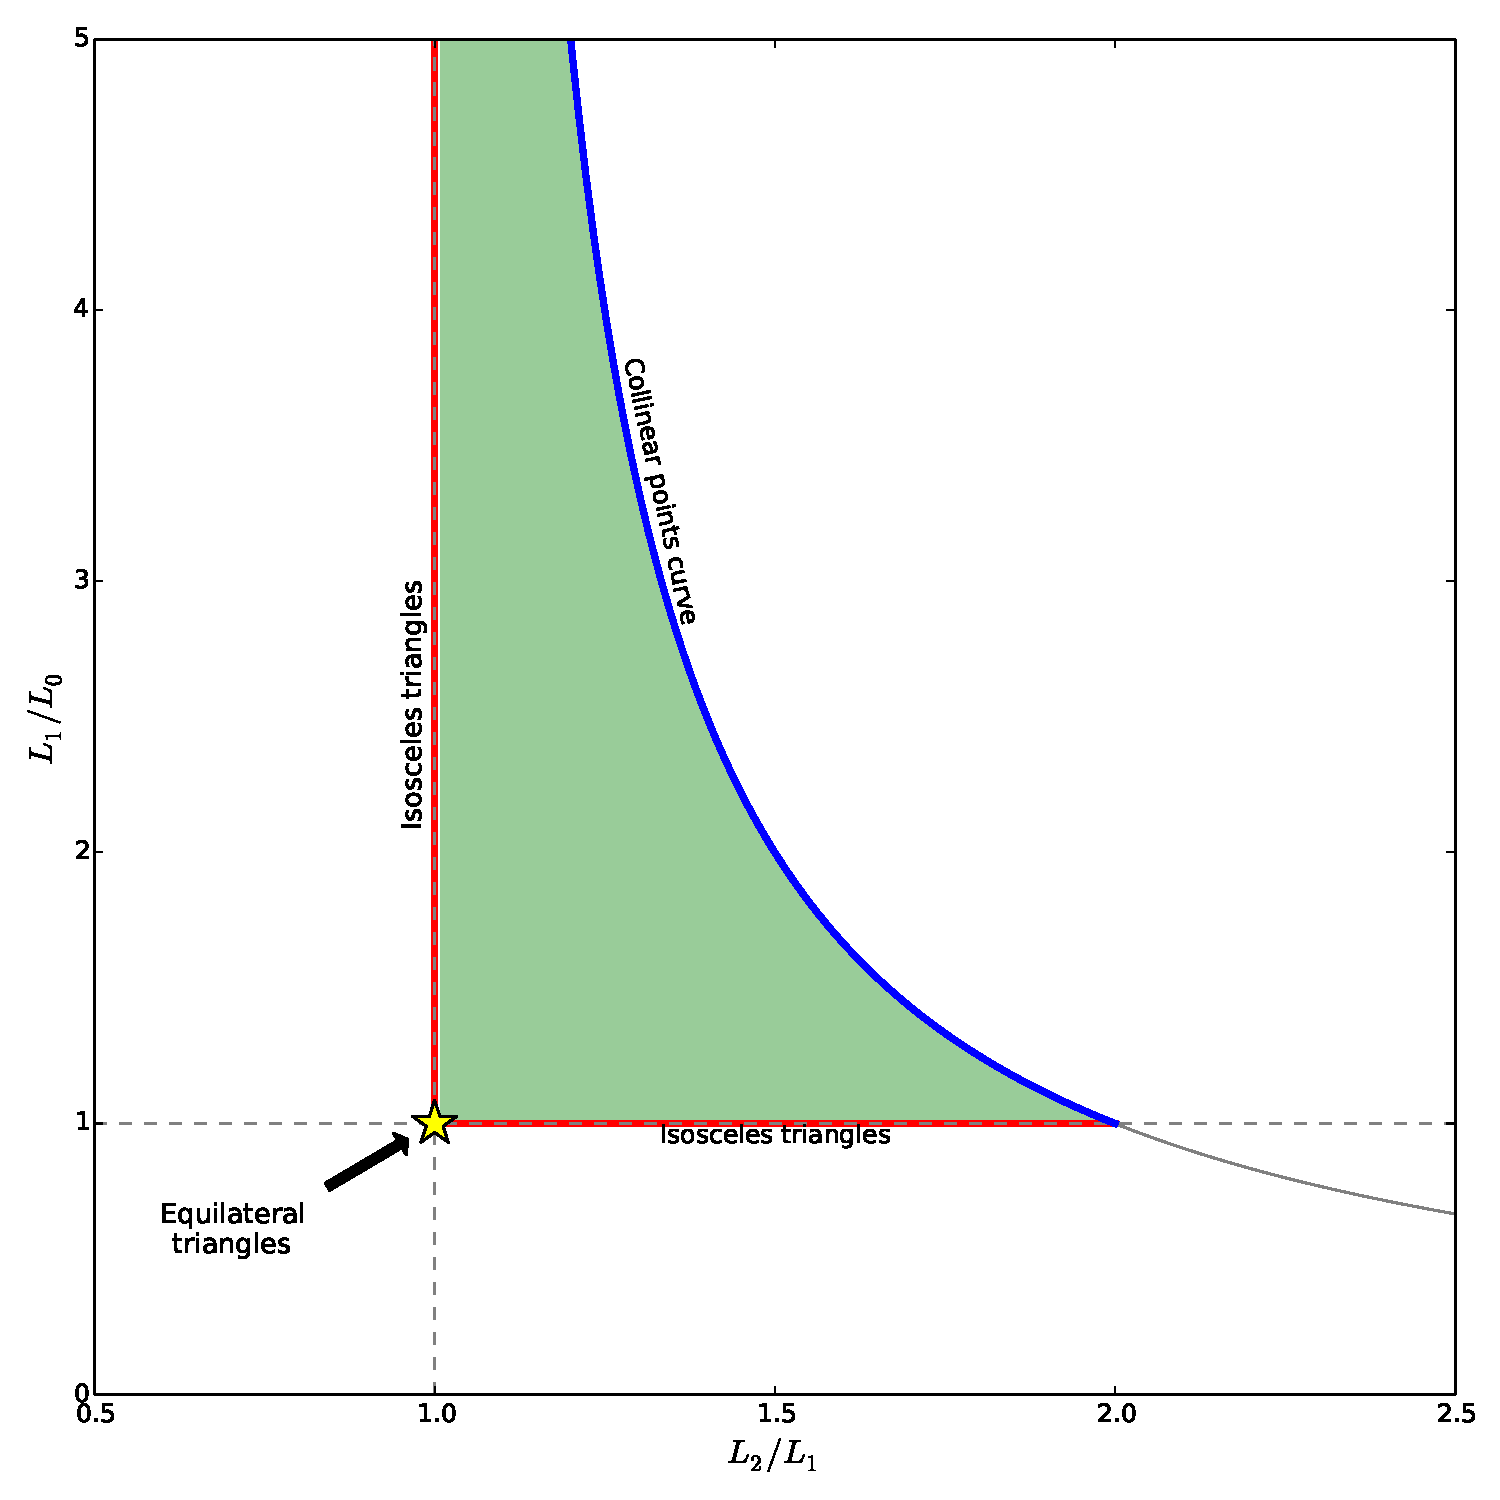
\includegraphics[width = \linewidth]{chapter_astroalign/figures/invariantMap01.pdf}
   \caption{Region for a particular invariant mapping}
   \label{fig:inv_region}
\end{figure}


%Other invariant sets can be constructed, each with a particular mapping from the set of side lengths of triangles to a region in the 2D plane of invariants.

%Some other examples are given in figure \ref{fig:inv_maps}. These have been explored numerically plotting the invariants for a large number of triangles.

%\begin{figure}[htb]
%   \centering
%   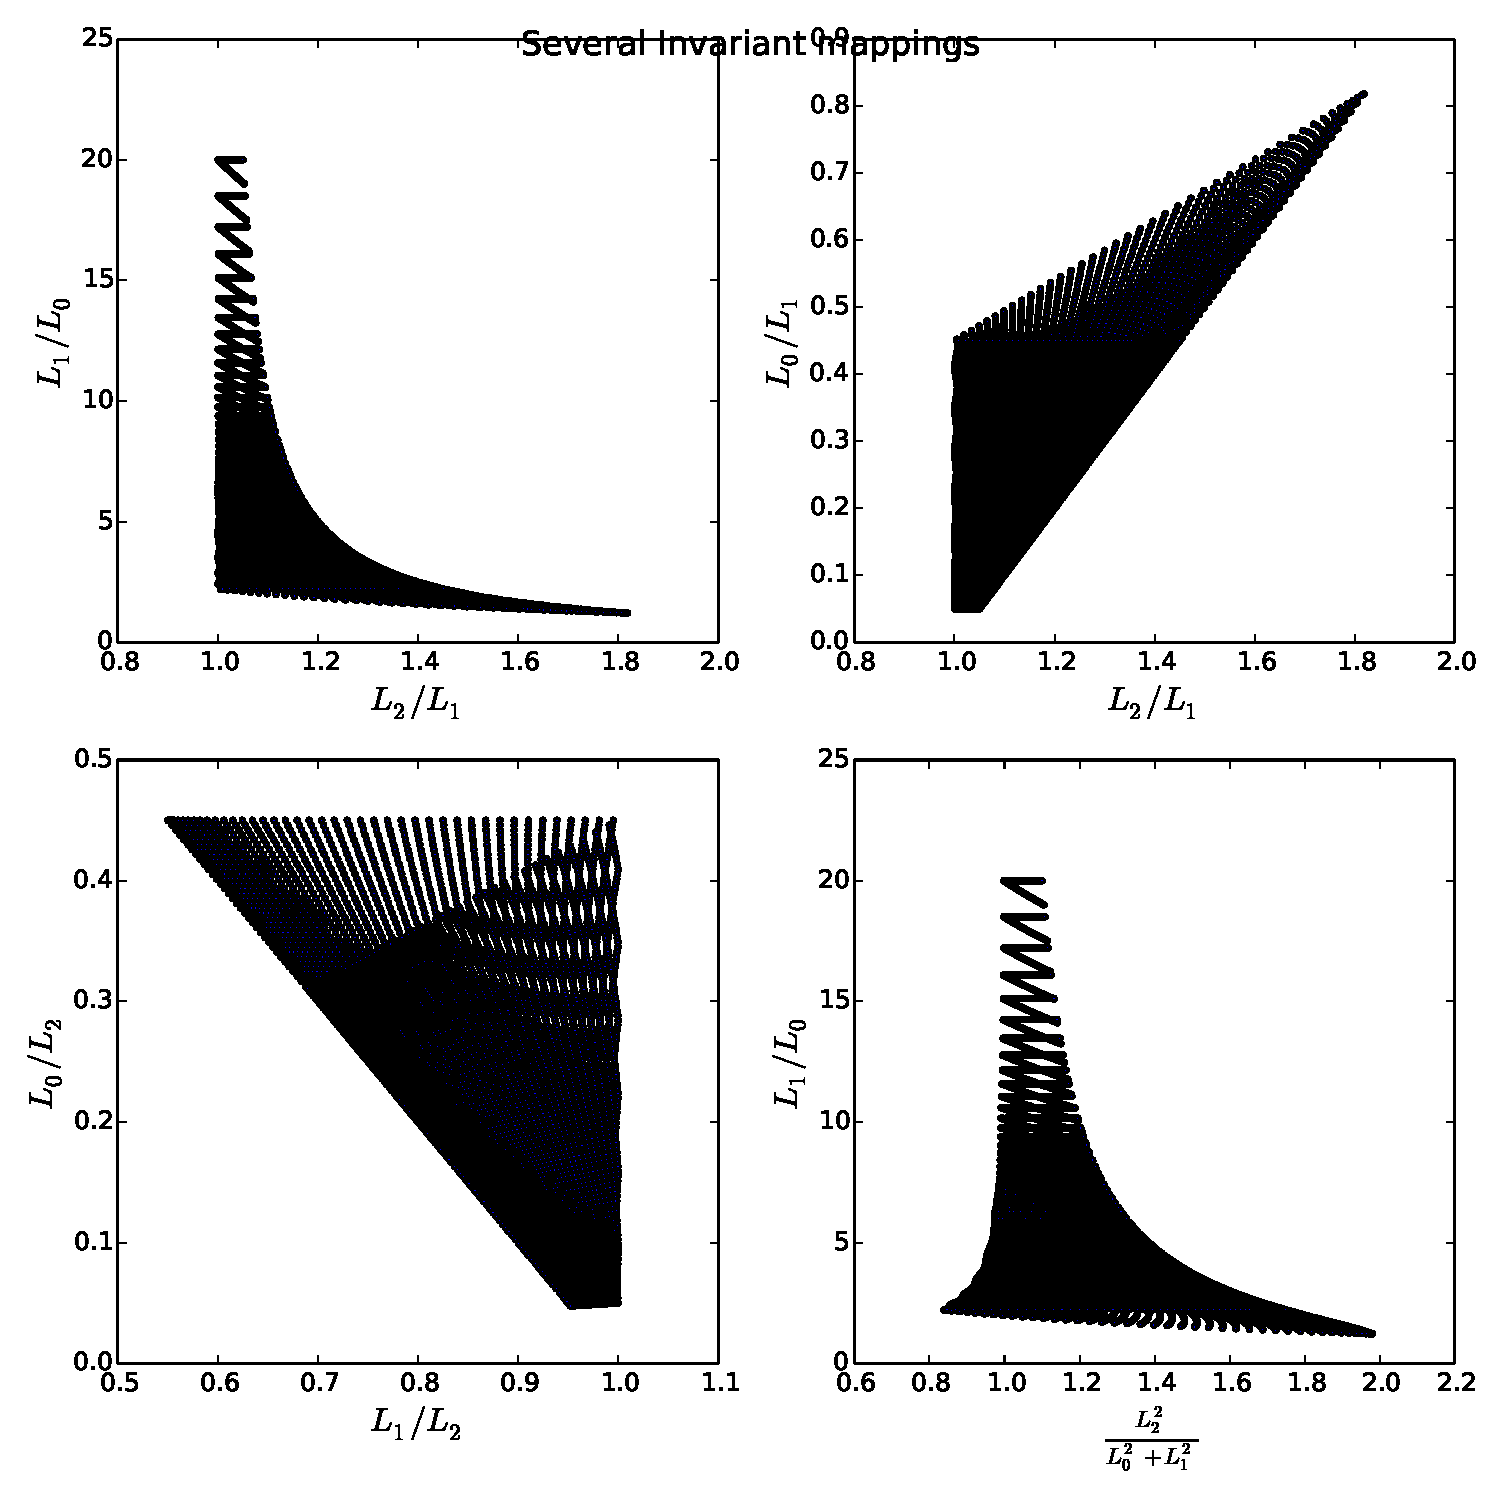
\includegraphics[width = \linewidth]{chapter_astroalign/figures/differentInvariantMaps.pdf}
%   \caption{Four examples of invariant mappings}
%   \label{fig:inv_maps}
%\end{figure}

%\lipsum

\subsection{An Ideal Example}

Let's see how the algorithm performs on an ideal example.

For this, we create several stars at random positions and we rotate and translate them as seen in figure \ref{fig:ideal_sources}.

\begin{figure}[htbp]
   \centering
   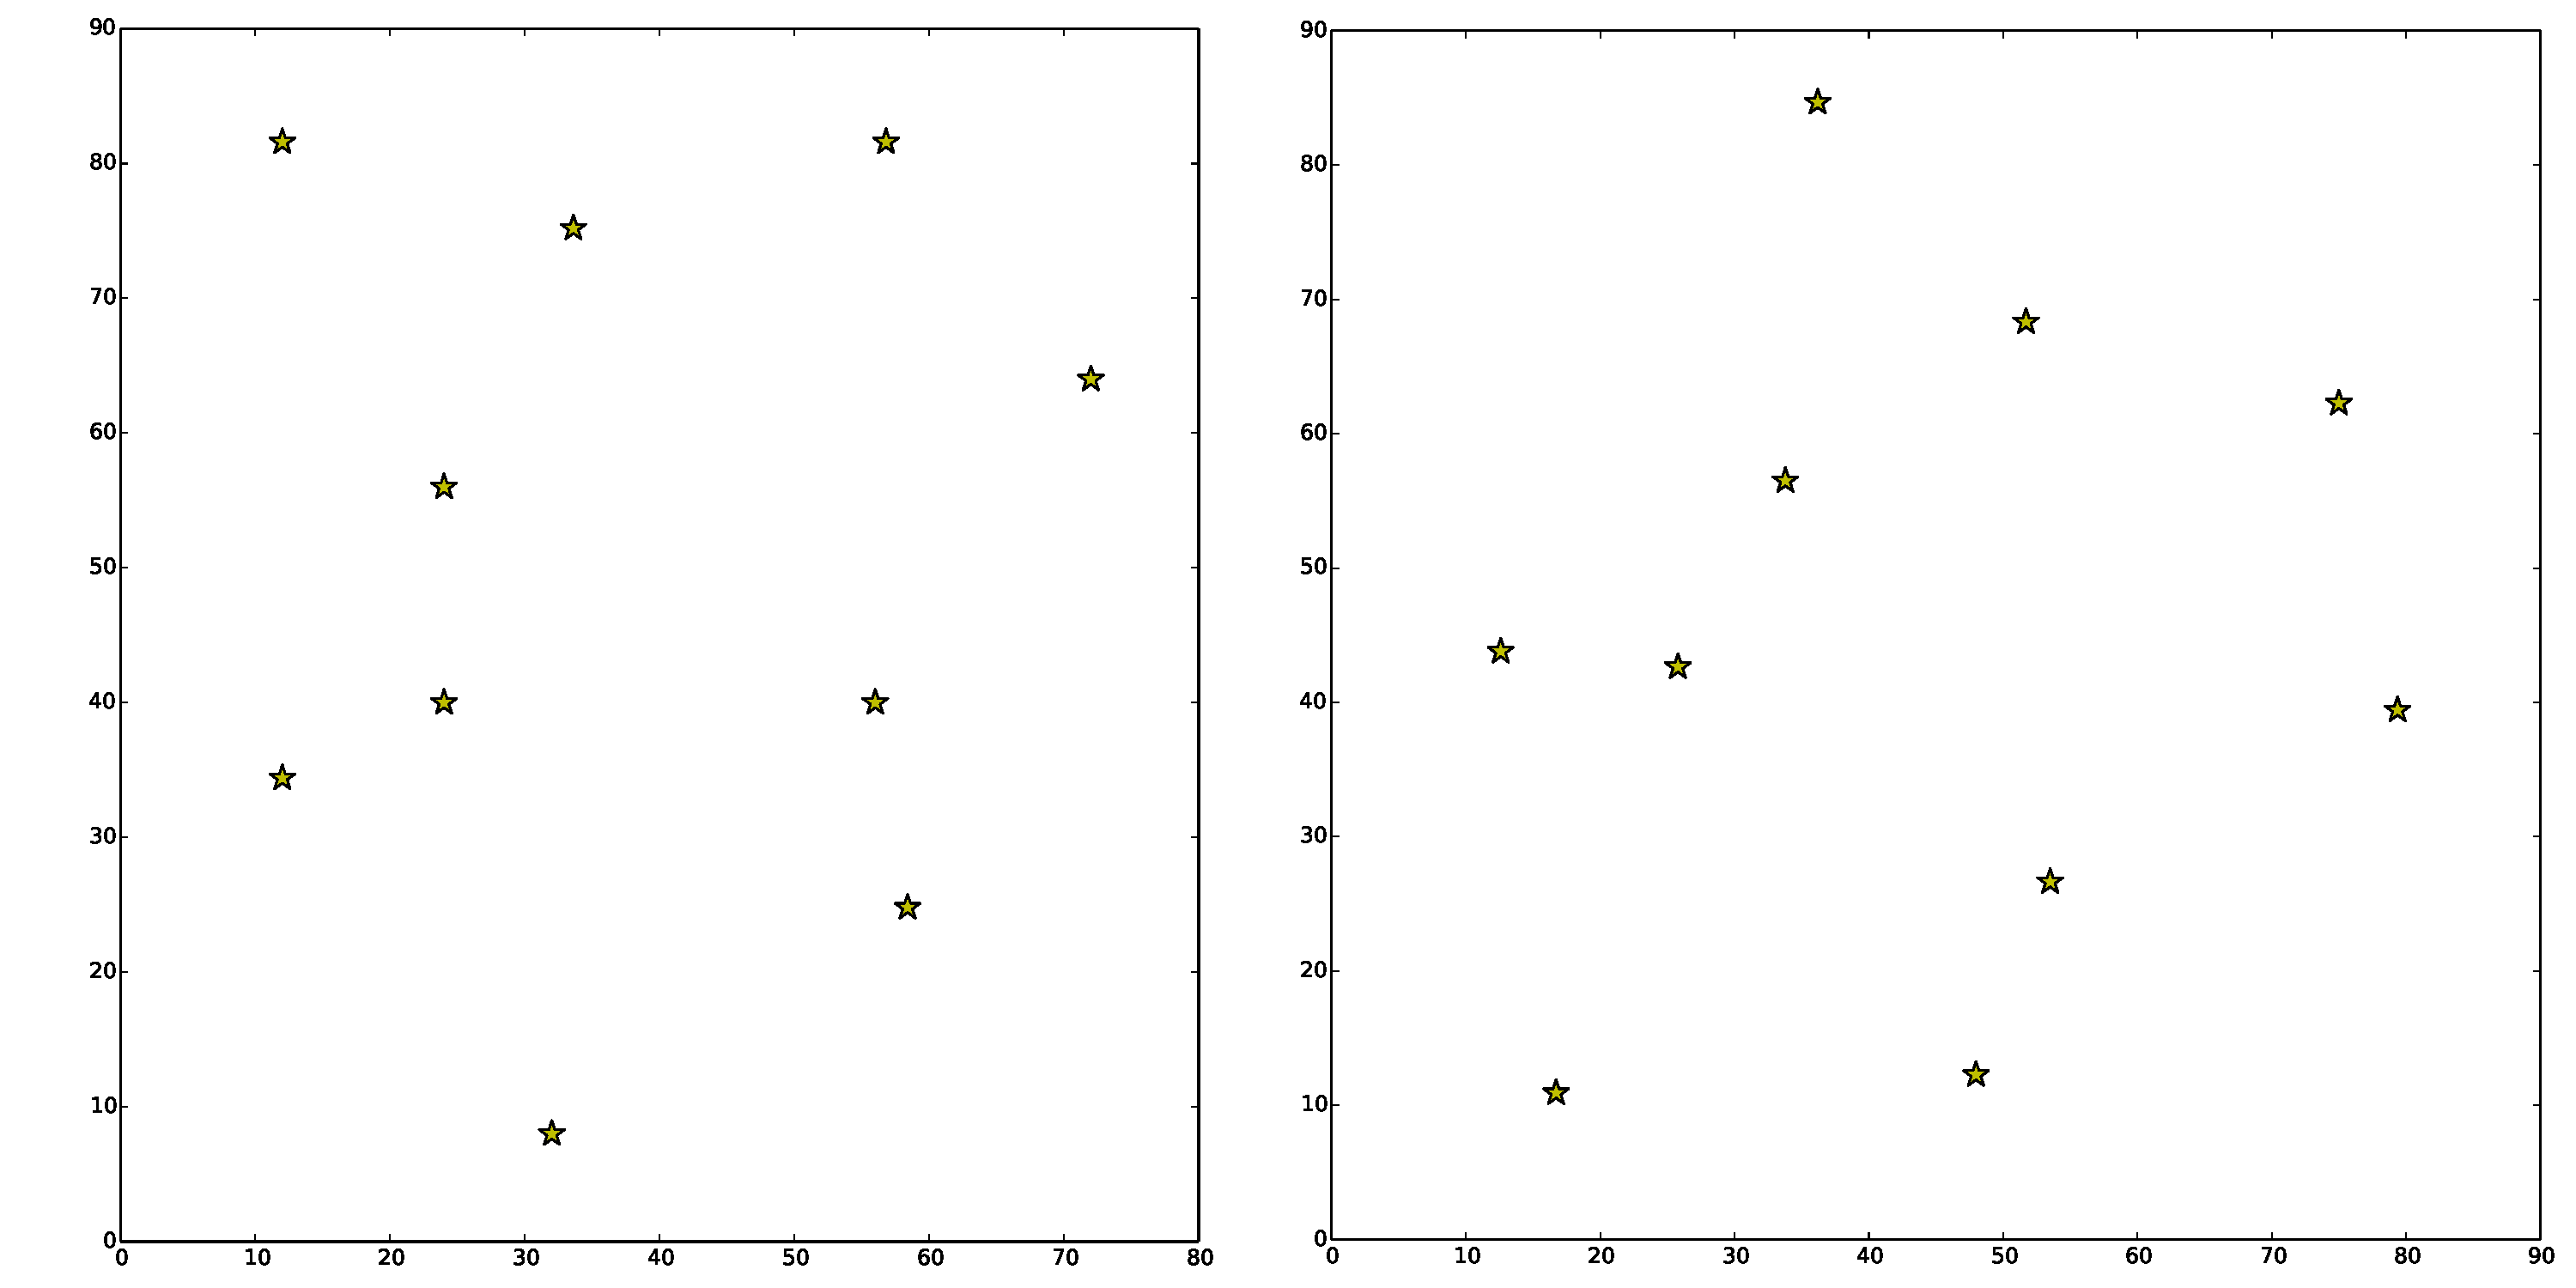
\includegraphics[width = \linewidth]{chapter_astroalign/figures/idealSources.pdf}
   \caption{Two ideal distribution of sources}
   \label{fig:ideal_sources}
\end{figure}

The invariant features in (\ref{inv01}) from this set of stars is plotted in figure \ref{fig:ideal_inv}.

\begin{figure}[htbp]
   \centering
   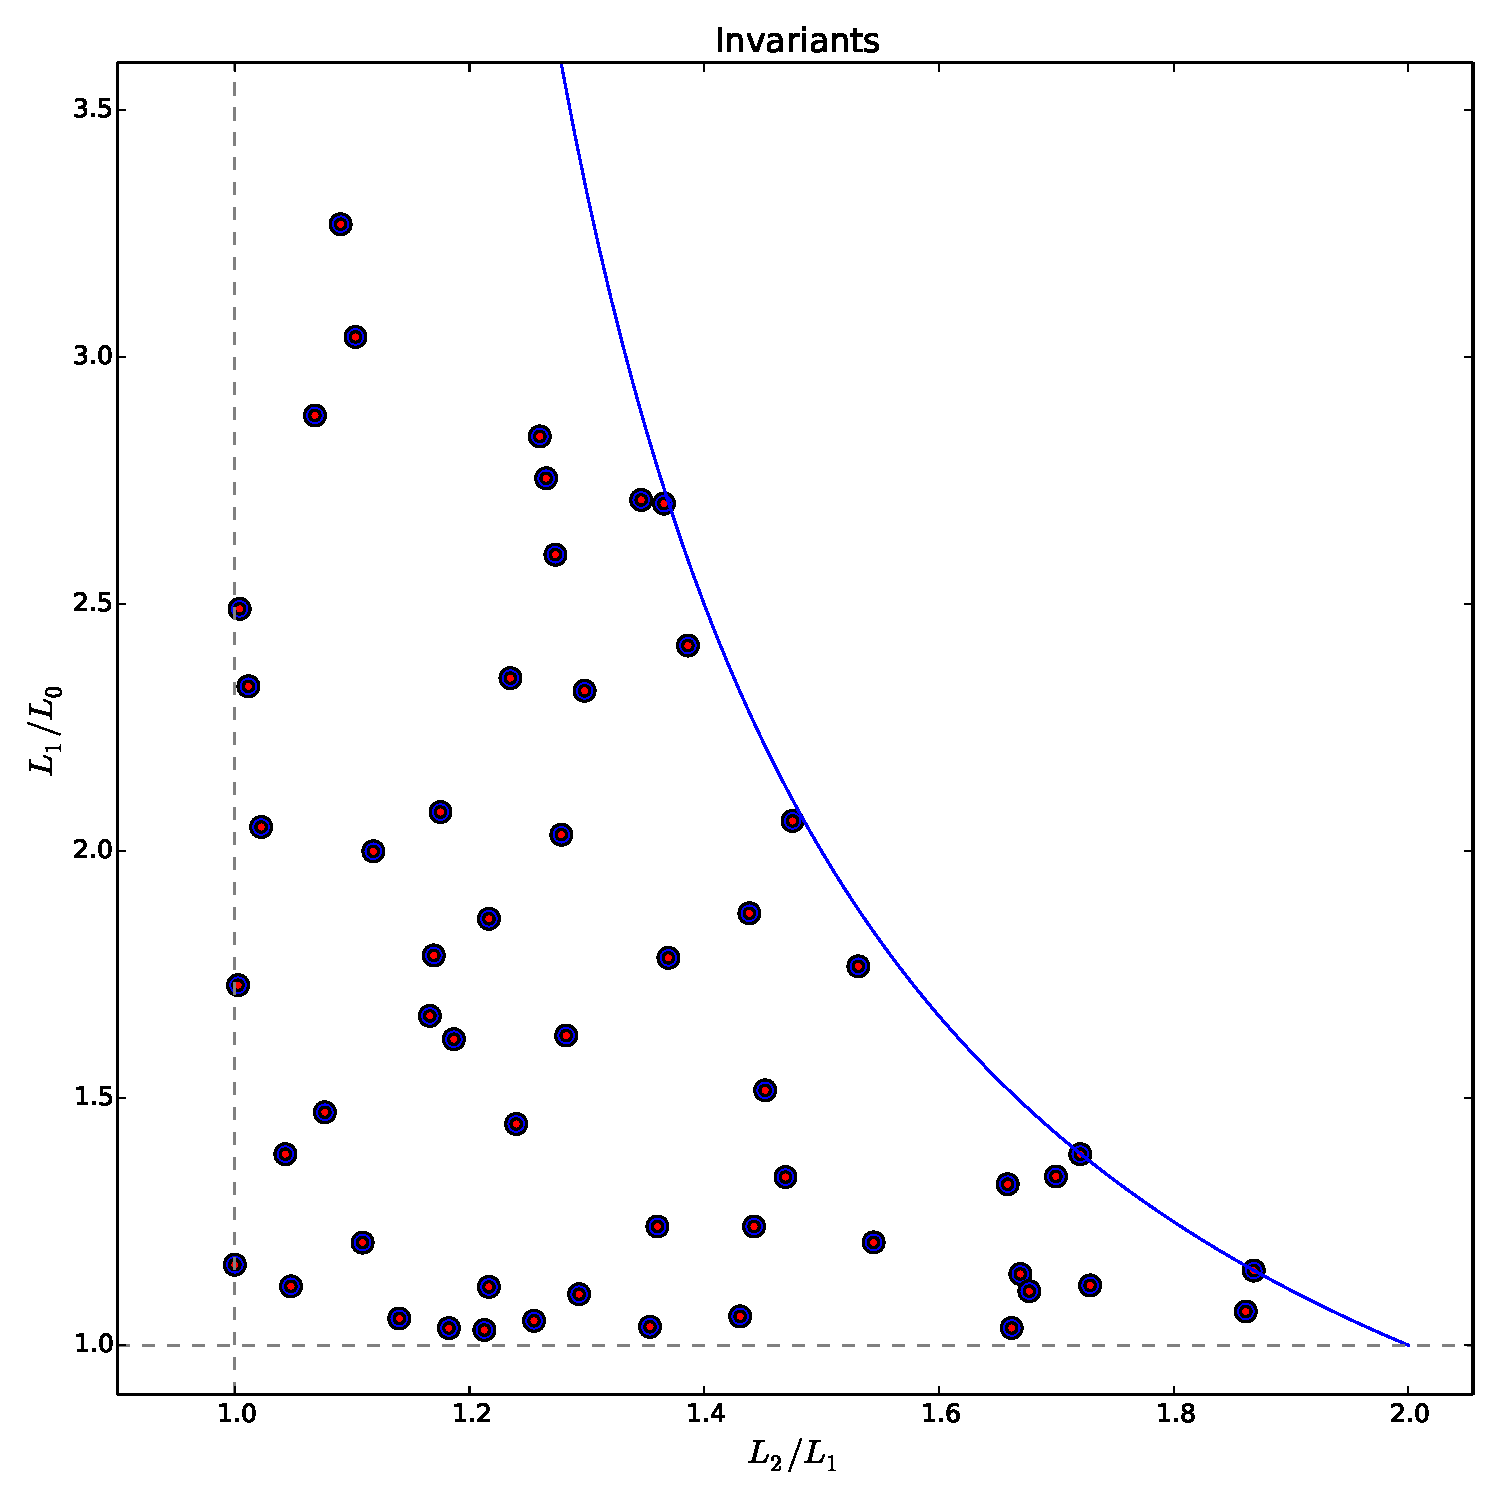
\includegraphics[width = \linewidth]{chapter_astroalign/figures/idealInvariants.pdf}
   \caption{Invariants for the ideal example}
   \label{fig:ideal_inv}
\end{figure}

We note that some invariants belong to collinear points, and the distribution of points is fairly sparse. 
This will help the identification phase when we try to match our triangles.

In the figure, the invariant points for both images were plotted. They appear superimposed in the plot.

We note that every blue invariant point has its corresponding red invariant point on top. 
There are no points without a partner for neither of the images. 
This is because all the sources in one image appear in the other one, there are no missing stars.
In a real situation, some stars will be missing because they are out of the field of view or because they became too faint due to extinction or any other technical reason. 
The algorithm should still work with missing or extra stars in the reference or test image. 

Another issue with real images is that locating the position of a source is not entirely precise, so small errors will appear in the expected position of one source with respect to its partner in the other image.
This error in turn creates an error on the lengths of the sides of the triangle and thus on the invariants calculated from it.
In practice, the invariant points will lay close to each other to a given small tolerance.

Once we have the set of invariants from both images, we query a correspondence to the kd-tree for possible matches within a given tolerance radius. 
Each returned match will be a correspondence between a triangle in one image and another. 
From each, we can make the point to point correspondence, provided all sides are unequal, and this will determine a unique transformation between the images.

Some of the correspondences won't be real ones. It could be that by chance there are two similar triangles in the images that belong to different set of stars.

This is where the RANSAC algorithm comes in.

\subsection{The RANSAC algorithm}

From its Wikipedia page 

{\em ``The Random sample consensus (RANSAC) algorithm is an iterative method to estimate parameters of a mathematical model from a set of observed data which contains outliers.''}

In our case the mathematical model is the similarity transformation between both images and the parameters are those of the transformation, i.e. the rotation, translation and uniform scaling parameters.

RANSAC is capable of choosing a transformation that fits most of the other triangles and is not affected by the rest of spurious outliers. 

This algorithm is also used in the computer vision package OpenCV for a very similar purpose, to ignore outliers when trying to estimate an homography between two images. 

In our case we look for the parameters $t_x$, $t_y$ for the translation in the $x$ and $y$ direction, the rotation angle $\alpha$ and the dilation parameter $\lambda$.

The transformation applied to a point $(x,y)$ will look like this:

\begin{align*}
\left(
 \begin{array}{lll} 
 \lambda \cos \alpha & \lambda \sin \alpha& \lambda t_x \\
 - \lambda \sin \alpha & \lambda \cos \alpha& \lambda t_y \\
 0 & 0 & 1
 \end{array}
\right)
\equiv
\left(
 \begin{array}{lll} 
 a_0 & b_0 & c_0 \\
-b_0 & a_0 & c_1 \\
 0 & 0 & 1
 \end{array}
\right)
\end{align*}

To make our problem linear, we will consider the parameters $a_0, b_0, c_0, c_1$ as if they were independent.

Two data points pairs are sufficient to determine uniquely a transformation for this 4 parameters. 
More can be used if we use a linear square minimization.

%This candidate transformation $T$ will be tested against all the other triangle matches in a RANSAC algorithm.

\subsection{Error propagation}

This is done by \citet{1995PASP..107.1119V}.



\section{Optimal Image Subtraction}
* Explanation Tools Developed (This would be a whole chapter)
	* Pipeline Framework (corral)
	* Reduction module for images
	* Spin-off packages relevant to the Python astronomical community: *astroalign* and *ois* (Optimal Image Subtraction, name can change in the future)
	
\chapter{Conclusions}
* The future of LIGO, TOROS and multi messenger astronomy


\appendix

\chapter{Notations }

Here we show the use of multiple appendixes.

\section{Math Notations}

Each appendix can have sub-sections as a regular chapter.


\section{Additional Notations}


\chapter{Ontologies}

These is another appendix.

\pagebreak{}

\bibliographystyle{plain}
\nocite{*}
\bibliography{sampleThesis}

\begin{vita}
This should be a one-page short vita.

There can be more paragraphs.\end{vita}

\end{document}
